% =====================================================================
%  The electronic component of cosmic rays as an ionizing agent of the
%  intergalactic medium during the epoch of reionization
%
%  Compile with:  pdflatex manuscript && bibtex manuscript && pdflatex x2
% =====================================================================
\documentclass[twocolumn]{article}

\usepackage[T1]{fontenc}
\usepackage[utf8]{inputenc}
\usepackage{amsmath,amssymb}
\usepackage{graphicx}
\usepackage{natbib}
\usepackage{booktabs}
\usepackage[margin=2.1cm]{geometry}
\usepackage{siunitx}
\usepackage[colorlinks=true,citecolor=blue,linkcolor=blue,
            urlcolor=blue]{hyperref}

\bibliographystyle{plainnat}

\newcommand{\Ke}{K_{\mathrm{e}}}
\newcommand{\Kini}{K_{\mathrm{ini}}}
\newcommand{\zi}{z_{\mathrm{i}}}
\newcommand{\xHI}{x_{\mathrm{HI}}}
\newcommand{\Msun}{M_{\odot}}

\title{\bf The electronic component of cosmic rays as an ionizing agent
of the intergalactic medium during the epoch of reionization}

\author{%
  \\[2pt]
  \small \textit{Draft manuscript}
}

\date{\today}

% =====================================================================
\begin{document}
\maketitle

\begin{abstract}
\noindent
Cosmic rays accelerated by the first stellar populations are injected into a
predominantly neutral intergalactic medium (IGM) at the same epoch during which
that medium is being reionized. We follow the kinetic energy $\Ke$ of a
cosmic-ray electron injected at $\zi = 20$ and $\zi = 10$ down to $z = 5.5$,
integrating simultaneously the seven relevant loss channels --- adiabatic
expansion, synchrotron, inverse Compton on the cosmic microwave background
(CMB) with the exact Klein--Nishina kernel, Coulomb scattering on the residual
plasma, collisional excitation and collisional ionization of neutral hydrogen,
and bremsstrahlung. We show that the $(z,\Ke)$ plane partitions into four
regimes separated by boundaries that we compute rather than assume:
$K_1 = 13.6\ \mathrm{eV}$, below which only Coulomb heating operates;
$K_2 = 7.6\times10^{4}$--$1.8\times10^{5}\ \mathrm{eV}$, where collisional
ionization gives way to inverse Compton; $K_3 = 4.2$--$7.9\ \mathrm{MeV}$,
above which the up-scattered CMB photons become ionizing; and
$K_4 = 3.2$--$4.3\times10^{8}\ \mathrm{eV}$, above which those photons
free-stream because their mean free path exceeds the Hubble radius. Solving the ionization
cascade self-consistently --- every generation of the secondary shower
integrated along its own trajectory, with the energy-dependent
binary-encounter-dipole secondary spectrum --- we find that the yield $Y$ per
injected electron is strongly non-linear in $\Kini$: the derived
$W = \Kini/Y$ has a broad minimum of $35.4\ \mathrm{eV}$ near
$1\ \mathrm{keV}$, where the deposition fractions
$(f_{\mathrm{ion}}, f_{\mathrm{exc}}, f_{\mathrm{heat}}) = (0.38, 0.42, 0.19)$
reproduce the $x_e\rightarrow0$ Monte Carlo limit, but rises to
$208\ \mathrm{eV}$ at $1\ \mathrm{MeV}$ and $\sim\!10^{8}\ \mathrm{eV}$ at
$1\ \mathrm{TeV}$, so no constant $W$ describes the yield. $Y$ flattens at
$7.7\times10^{3}$ ($\zi=20$) and $1.2\times10^{4}$ ($\zi=10$)
for $\Kini \gtrsim 10^{8}\ \mathrm{eV}$: above $K_4$ every additional electron
volt is radiated into photons that leave the medium. The four boundaries divide
the leptonic contribution into two productive bands separated by a dead one:
direct collisional ionization below $K_2$, a band $K_2 < \Ke < K_3$ in which
inverse Compton dominates but the up-scattered photons fall below the
ionization threshold and the energy is lost to the sub-ionizing background, a
second productive band $K_3 < \Ke < K_4$ in which those photons are ionizing
and are absorbed locally, and outright escape above $K_4$. Because a
diffusive-shock-acceleration spectrum places most of its energy above $K_4$,
the leptonic component is an intrinsically inefficient reionizing agent unless
the injection spectrum is soft.
\end{abstract}

\smallskip
\noindent\textbf{Key words:} intergalactic medium -- dark ages, reionization,
first stars -- cosmic rays -- radiation mechanisms: non-thermal

% =====================================================================
\section{Introduction}
% =====================================================================

\subsection{The epoch of reionization}

The epoch of reionization (EoR) is the last global phase transition of the
baryonic Universe: the moment at which the intergalactic hydrogen left neutral
by cosmological recombination was returned to an ionized state by the first
luminous sources. Its end point is now pinned down with some precision. The
distribution of effective optical depths in the \mbox{Lyman-$\alpha$} forest of
the XQR-30 quasar sample requires that reionization-related fluctuations --- in
the ultraviolet background, in the residual neutral fraction, or in the IGM
temperature --- persist until at least $z = 5.3$, so that the process cannot
have finished appreciably earlier \citep{Bosman2022}. At the other end, the
Thomson optical depth to the CMB measured by \emph{Planck},
$\tau = 0.054 \pm 0.007$, places the midpoint of a rapid transition near
$z \simeq 7.7$ and disfavours a substantial ionized fraction before
$z \sim 15$ \citep{Planck2020}. The interval $5.5 \lesssim z \lesssim 20$
adopted throughout this work therefore brackets the entire transition together
with the preceding era in which the first sources were already operating.

What is far less settled is the \emph{photon budget}: which sources supplied
the ionizing photons, and whether they supplied enough of them at the right
time. Star-forming galaxies are the standard answer \citep{Robertson2022}, but
the \emph{James Webb Space Telescope} has complicated it rather than closed it.
The abundance and ionizing efficiency $\xi_{\mathrm{ion}}$ inferred for early
galaxies are high enough that, taken at face value with canonical escape
fractions, they would complete reionization too early and overshoot both the
CMB and the \mbox{Lyman-$\alpha$} forest constraints --- a tension now referred
to as the photon budget crisis \citep{Munoz2024}. A budget that is
simultaneously over-supplied in photons and under-constrained in timing is
precisely the situation in which secondary, non-stellar ionizing channels
deserve to be quantified rather than assumed negligible. The purpose of this
paper is to quantify one such channel from first principles.

\subsection{Cosmic dawn}

Reionization does not begin with reionization. It begins with cosmic dawn, the
interval during which the first collapsed structures light up and start
depositing energy in a medium that is still almost fully neutral. The
observational handle on this era is the redshifted 21-cm line, and it has
recently become quantitative: the HERA Phase~I power-spectrum limits require
that the IGM was heated above the adiabatic cooling floor no later than
$z = 10.4$, which rules out the whole family of ``cold reionization''
histories in which the gas remains at its adiabatic temperature until
ionization fronts arrive \citep{HERA2023}. Something was already injecting
energy into the neutral IGM well before the ionized bubbles overlapped.

That early energy injection is what makes cosmic dawn the natural starting
point of the present analysis. Whatever heats the IGM at $z \sim 10$--$20$ must
do so by depositing the kinetic energy of some non-thermal particle population
into a gas of density
$n_{\mathrm{HI}} \simeq 2.6\times10^{-4}$--$1.8\times10^{-3}\ \mathrm{cm^{-3}}$,
and the same deposition that raises the temperature will, above the appropriate
threshold, also produce free electrons. The heating and ionization channels are
not independent: they are two branches of the same energy-loss problem, and
they are set by the same cross-sections. The HERA constraint tells us the
heating branch was active; the question this paper addresses is how much of the
same energy budget could have gone into the ionization branch.

\subsection{The first stellar populations}

The sources responsible are the first stellar populations. Metal-free Pop~III
stars form in minihaloes of
$\sim\!10^{5}$--$10^{6}\,\Msun$ from $z \sim 30$ onwards; primordial gas is
strongly susceptible to fragmentation, so they form in small clusters with a
roughly logarithmically flat mass function extending to several tens of solar
masses, and feedback from the most massive members regulates all subsequent
star formation \citep{Klessen2023}. These stars are short-lived, and a large
fraction of them end as core-collapse supernovae within a few million years of
formation --- on a timescale much shorter than the $\sim\!290\ \mathrm{Myr}$
that separates $z = 20$ from $z = 10$ in the adopted cosmology.

The relevance of this population to the present problem is that it delivers,
in a single stellar generation, all four of the astrophysical engines known to
accelerate particles to relativistic energies: fast radiatively driven and
rotationally driven stellar winds, supernova blast waves, accreting compact
objects in high-mass X-ray binaries (HMXBs), and the magnetized rotators left
behind by the explosions. Each of these operates in an environment that is
poorer in metals and, plausibly, richer in magnetic energy per unit mass than
its low-redshift counterpart, and each of them terminates in a shock or a
magnetosphere in which charged particles are accelerated out of the thermal
pool. The first stellar populations are, in other words, the first cosmic-ray
sources.

\subsection{Winds, supernovae, HMXBs and compact remnants}

Of these engines the supernova blast wave is the best characterized. Particle
acceleration at non-relativistic quasi-parallel collisionless shocks proceeds
through diffusive shock acceleration (DSA), and kinetic particle-in-cell
simulations now show that protons \emph{and} electrons are accelerated
simultaneously at such shocks, both developing power-law momentum distributions
with the universal DSA index $-4$, corresponding to
$\mathrm{d}N/\mathrm{d}K \propto K^{-2}$ in the relativistic limit
\citep{Park2015}. The same simulations, together with the observed
$\sim\!1\%$ electron fraction of the local Galactic cosmic-ray flux near a
GeV, motivate an electron-to-proton number ratio $K_{e/p} \sim 10^{-2}$ at
injection. High-mass X-ray binaries contribute along a different route: their
X-ray output scales inversely with metallicity, so the metal-poor systems
characteristic of early galaxies are expected to be substantially more
luminous per unit star formation than local analogues \citep{Kaur2022}, and the
same accretion-powered outflows that produce that X-ray emission are efficient
particle accelerators. Taken together these engines make early star-forming
galaxies copious cosmic-ray sources \citep{Owen2017,Ruszkowski2023}.

The crucial step for what follows is escape. A cosmic ray produced inside a
minihalo only matters for the IGM if it leaves the halo, and low-mass haloes
are poorly equipped to confine it: their escape velocities and magnetic
confinement times are small, and the photoevaporation that accompanies the
first ionizing sources removes much of the confining gas. Low-energy cosmic
rays produced by Pop~III supernova remnants are therefore expected to be
released more or less directly into the surrounding neutral IGM, and this is
the configuration assumed by essentially all subsequent treatments of
cosmic-ray feedback at high redshift \citep{Sazonov2015,Leite2017,Jana2018}. We
adopt it here: the electron whose history we integrate is one that has already
escaped its host halo and finds itself in the diffuse IGM at redshift $\zi$.

\subsection{Cosmic rays in the early intergalactic medium}

The idea that this escaped population might matter cosmologically is not new.
\citet{Nath1993} asked directly whether cosmic rays from young galaxies could
reionize the IGM, and the question has been revisited repeatedly since, with
progressively more complete microphysics
\citep{Samui2005,Sazonov2015,Leite2017,Jana2018,Bera2023,GesseyJones2023}. The
modern consensus is sharply asymmetric between the two branches identified
above. On the heating side the effect is real and substantial: cosmic rays from
primordial supernovae can raise the IGM above the CMB temperature by
$z \sim 15$ (Pop~III) or $z \sim 10$ (Pop~II) \citep{Sazonov2015}, and
detailed transport calculations give $\Delta T \simeq 10$--$200\ \mathrm{K}$ by
$z = 10$ depending on the injection spectrum \citep{Leite2017}. Because the
heating is short-ranged and clustered around star-forming sites it also leaves
a distinctive small-scale signature in the 21-cm power spectrum that
distinguishes it from X-ray heating \citep{GesseyJones2023}, although for
typical diffusion coefficients the heating becomes effectively uniform at high
redshift \citep{Jana2018}.

On the ionization side the same literature concludes that the contribution is
negligible \citep{Leite2017}. That conclusion, however, has almost invariably
been reached for the \emph{hadronic} component, and for good reason: cosmic-ray
protons carry the bulk of the energy budget, and their Coulomb and ionization
losses in a neutral medium are the natural first thing to compute. The
electronic component has received far less attention, even though it interacts
with the medium through a completely different set of channels --- inverse
Compton scattering on the CMB in particular, which at fixed total energy is
suppressed for protons by $(m_e/m_p)^{4} \simeq 10^{-13}$ and is therefore
irrelevant, but which for electrons at these
redshifts dominates everything else above $\sim\!100\ \mathrm{keV}$. Whether
the negligible-ionization verdict carries over to the leptonic component is not
obvious \emph{a priori}, and it is the question we set out to answer.

\subsection{Scope: the leptonic component}

We therefore restrict this paper to the electronic component of the cosmic-ray
flux and defer the hadronic branch entirely. This is a deliberate separation
rather than an omission. Cosmic-ray protons at these energies lose energy
through Coulomb collisions and hadronic $pp$ interactions, the latter producing
pions whose decay injects secondary $e^{\pm}$ and $\gamma$-rays; those
secondaries re-enter the same leptonic cascade we analyse here, so the
per-electron yields computed below are exactly the quantities a subsequent
hadronic calculation would need as input. Separating the two also keeps the
uncertainties separate: the leptonic problem is governed by cross-sections that
are known to better than a few per cent, whereas the hadronic branch carries
the additional uncertainty of the pion multiplicity and the proton spectrum.
The hadronic contribution will be treated in a companion paper.

Within this scope our strategy is to compute everything \emph{per injected
electron}, as a function of the injection energy $\Kini$ and the injection
redshift $\zi$, and to postpone any convolution with a source spectrum to the
very end. The per-electron yield is a property of the IGM and of atomic
physics alone; the source spectrum is a property of the accelerator, and it is
by far the more uncertain of the two. Presenting the results in this order
means that the central results of this paper --- the boundaries of the four
regimes and the ionization yield curve --- remain valid regardless of what is
eventually assumed about the accelerators, and that a reader with a different
spectrum in mind can re-weight our curves without repeating the integration.

% =====================================================================
\section{Energy losses of an electron in the intergalactic medium}
\label{sec:method}
% =====================================================================

\subsection{Fiducial medium and the seven loss channels}

We adopt a spatially uniform, pure-hydrogen IGM with
$n_{\mathrm{HI}}(z) = 1.8\times10^{3}\,[(1+z)/21]^{3}\ \mathrm{m^{-3}}$
(that is, $1.8\times10^{-3}$, $2.6\times10^{-4}$ and
$5.3\times10^{-5}\ \mathrm{cm^{-3}}$ at $z = 20$, $10$ and $5.5$), a residual
ionized fraction $x_e = n_e/n_{\mathrm{HI}} = 10^{-4}$, and a magnetic field
frozen into the expansion, $B(z) = B_0 (1+z)^{2}$ with $B_0 = 1\ \mathrm{nG}$
comoving. Cosmological quantities use the \emph{Planck} 2018 parameters
\citep{Planck2020} as tabulated in \texttt{astropy} \citep{Astropy2022}; in
this cosmology $z = 20$, $10$ and $5.5$ correspond to cosmic ages of $178.1$,
$471.4$ and $1038.5\ \mathrm{Myr}$. Helium is neglected, which is conservative
for the ionization yields quoted below.

Seven loss channels act on the electron simultaneously, and we integrate them
together rather than in the more usual sequential approximation. Adiabatic
losses follow $\dot K = -H(z)\,p^{2}c^{2}/E$. Synchrotron and inverse Compton
losses are treated in the same isotropic-pitch-angle form,
$\dot K = -\tfrac{4}{3}\sigma_{\mathrm{T}} c\,U\,(p^{2}c^{2}/E_0^{2})$, with
$U = U_B$ and $U = U_{\mathrm{CMB}} F_{\mathrm{KN}}(b)$ respectively, where
$F_{\mathrm{KN}}$ is the exact Klein--Nishina kernel integrated over the Planck
spectrum \citep{Blumenthal1970} and $b = 4\gamma k T_{\mathrm{CMB}}(z)/E_0$.
Coulomb losses on the residual plasma follow \citet{Gould1972} with maximum
fractional transfer $\delta = 0.5$. Collisional excitation
$\mathrm{H}(1s)\!\rightarrow\!\mathrm{H}(np)$ is summed over $n = 2$--$10$
using the scaled plane-wave Born cross-sections of \citet{Stone2002}, and
collisional ionization uses the relativistic binary-encounter-Bethe (RBEB)
cross-section of \citet{Kim2000}, with the energy lost per ionizing collision
taken as the binding energy plus the mean secondary energy. Bremsstrahlung on
neutral and ionized hydrogen follows \citet{Blumenthal1970} with a continuous
interpolation between the screened and unscreened limits.

\subsection{The magnetic field is dynamically irrelevant}

One consequence of the fiducial choice deserves to be stated at the outset,
because it simplifies the entire analysis. Since both $U_B$ and
$U_{\mathrm{CMB}}$ scale as $(1+z)^{4}$, their ratio is a redshift-independent
constant, and for $B_0 = 1\ \mathrm{nG}$ it is
$U_B/U_{\mathrm{CMB}} = 9.5\times10^{-8}$. Synchrotron losses are therefore
about seven orders of magnitude below inverse Compton losses at \emph{every}
redshift and \emph{every} energy in our window; equipartition with the CMB
would require $B_0 \simeq 3.2\ \mathrm{\mu G}$ comoving, four orders of
magnitude above the fiducial value. The synchrotron channel is retained in the
integration for completeness but never affects any result reported here, and
this is a physical statement about the early IGM rather than a numerical
artefact.

The magnetic field nevertheless matters enormously for \emph{transport}, and in
the opposite direction. The gyroradius $r_g = p_\perp/(eB)$ at $z = 10$, where
the proper field is $121\ \mathrm{nG}$, is $1.3\times10^{-8}\ \mathrm{pc}$ for
a $1\ \mathrm{MeV}$ electron and only $9\times10^{-3}\ \mathrm{pc}$ even at
$1\ \mathrm{TeV}$. Compared with the tens of comoving megaparsecs of path
length that the same electron traverses before thermalizing
(Sect.~\ref{sec:shell}), the electron is tied to its field line to one part in
$10^{10}$. Any statement about \emph{where} the ionizations occur is therefore
a statement about cosmic-ray transport, not about the loss physics; we return
to this point in Sect.~\ref{sec:shell}.

\subsection{Integration}

The seven rates are assembled into a single stiff ordinary differential
equation for $\Ke(t)$, integrated with an implicit Radau scheme from the
cosmic time corresponding to $\zi$ down to $z = 5.5$, with a terminal event
that stops the integration when the electron reaches the thermal floor
$K_{\mathrm{term}} = \tfrac{3}{2} k T_{\mathrm{CMB}}(z)$. To obtain the energy
budget of each channel separately we integrate an augmented eight-state system
that carries the seven cumulative integrals $\int L_i\,\mathrm{d}t$ alongside
$\Ke$; this guarantees that the channel budgets are evaluated on the true
trajectory rather than on an approximate one, and that they sum to
$\Kini - \Ke(t)$ by construction. The ionization yield of
Sect.~\ref{sec:cold} is obtained from two further augmented states carrying the
primary collision count $\int n_{\mathrm{HI}} v \sigma_{\mathrm{ion}}\,
\mathrm{d}t$ and the cascade total of Eq.~(\ref{eq:cascade}), so that the
number of ionizations and the energy lost to them are computed from the same
cross-section on the same trajectory.

Figure~\ref{fig:rates} shows the resulting loss rates at $z = 20$ and
$z = 10$. The structure is the same at both redshifts and is what organizes the
rest of this paper: a Coulomb-dominated regime at the lowest energies, a broad
plateau in which collisional ionization of neutral hydrogen carries the losses,
and a steeply rising inverse-Compton regime above it in which the total rate
grows as $\Ke^{2}$. Adiabatic, synchrotron and bremsstrahlung losses never
dominate anywhere in the plane; the peak fractional contribution of the
adiabatic term over the whole window is $\lesssim\!0.09$, reached for
$\Kini \sim 10^{6}\ \mathrm{eV}$ at $\zi = 10$ (Fig.~\ref{fig:budget}).

\begin{figure*}[t]
\centering
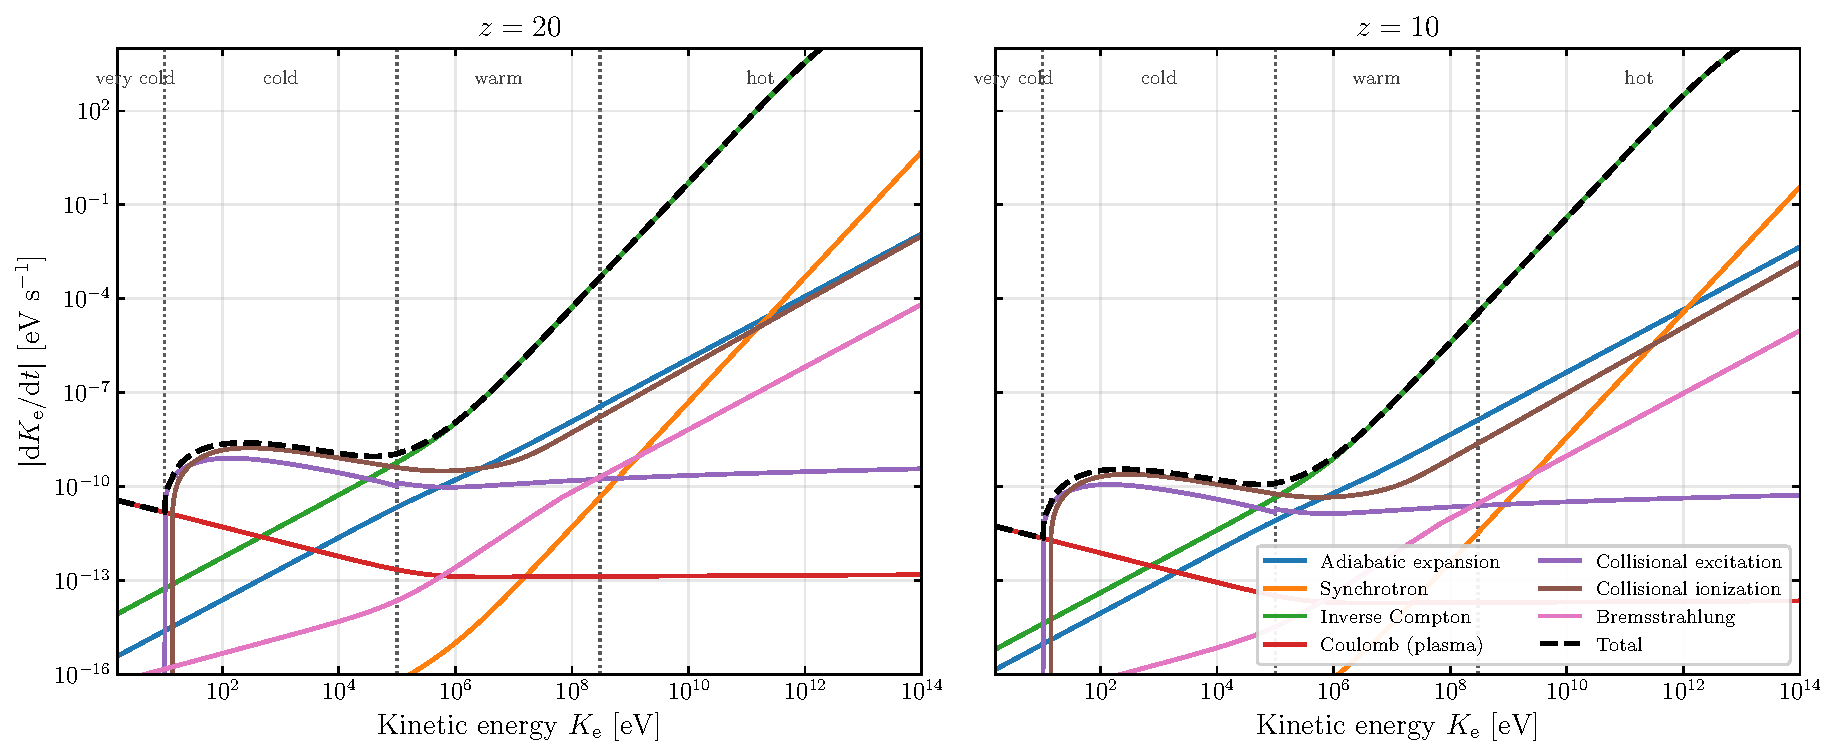
\includegraphics[width=\textwidth]{figures/fig01_loss_rates.pdf}
\caption{Energy-loss rate $|\mathrm{d}\Ke/\mathrm{d}t|$ of a cosmic-ray
electron in the fiducial IGM, decomposed into the seven channels, at $z = 20$
(left) and $z = 10$ (right). The dotted vertical lines mark the nominal
boundaries of the four regimes of the conceptual scheme ($10.2\ \mathrm{eV}$,
$100\ \mathrm{keV}$, $300\ \mathrm{MeV}$); the boundaries computed in
Sect.~\ref{sec:bins} are given in Table~\ref{tab:bins}. Synchrotron losses lie
$\sim\!7$ orders of magnitude below inverse Compton at all energies because
$U_B/U_{\mathrm{CMB}} = 9.5\times10^{-8}$ for $B_0 = 1\ \mathrm{nG}$ comoving.}
\label{fig:rates}
\end{figure*}

% =====================================================================
\section{The four-regime partition of the $(z,\Ke)$ plane}
\label{sec:bins}
% =====================================================================

\subsection{Boundaries computed, not assumed}

The conceptual scheme underlying this work divides cosmic-ray electrons into
four classes --- very cold, cold, warm and hot --- on the basis of which
deposition channel their energy ultimately reaches. We can now replace those
nominal divisions by boundaries computed from the loss physics itself.
Figure~\ref{fig:phase} shows the dominant channel as a function of $(z,\Ke)$
over the full window $5.5 \le z \le 20$, with four boundary curves overlaid,
and Table~\ref{tab:bins} lists their values. The first, $K_1 = 13.61\
\mathrm{eV}$, is the hydrogen ionization threshold and is redshift-independent
by construction; below it no inelastic atomic channel is open and Coulomb
scattering on the residual plasma is the only sink. The second,
$K_2$, is the crossover at which the inverse-Compton rate overtakes the
collisional-ionization rate; it runs from $7.6\times10^{4}\ \mathrm{eV}$ at
$z = 20$ to $1.8\times10^{5}\ \mathrm{eV}$ at $z = 5.5$, bracketing the nominal
$100\ \mathrm{keV}$ division. Its mild redshift dependence has a transparent
origin: collisional losses scale as $n_{\mathrm{HI}} \propto (1+z)^{3}$ while
inverse Compton scales as $U_{\mathrm{CMB}} \propto (1+z)^{4}$, so the
crossover moves to lower energy as $z$ increases.

The remaining two boundaries are not properties of the electron's cooling at
all but of the \emph{fate of the photons it produces}, and they are the reason
the inverse-Compton regime must be subdivided. $K_3$ is the electron energy at
which the up-scattered CMB photons first reach the hydrogen ionization
threshold of $13.6\ \mathrm{eV}$; evaluating the exact head-on scattering
kinematics against the high-energy tail of the Planck spectrum (the $99$th
percentile of the CMB energy density, $x = h\nu/kT = 8.17$) gives
$K_3 = 4.20$, $5.99$ and $7.93\ \mathrm{MeV}$ at $z = 20$, $10$ and $5.5$.
Using instead the mean CMB photon, $x = 2.70$, raises these to $7.7$, $10.8$
and $14.2\ \mathrm{MeV}$, so the threshold is of order a few MeV with a
factor-of-two definitional spread. $K_4$ is the electron energy above which
those photons escape, and it is derived in Sect.~\ref{sec:hot}.

\begin{figure*}[t]
\centering
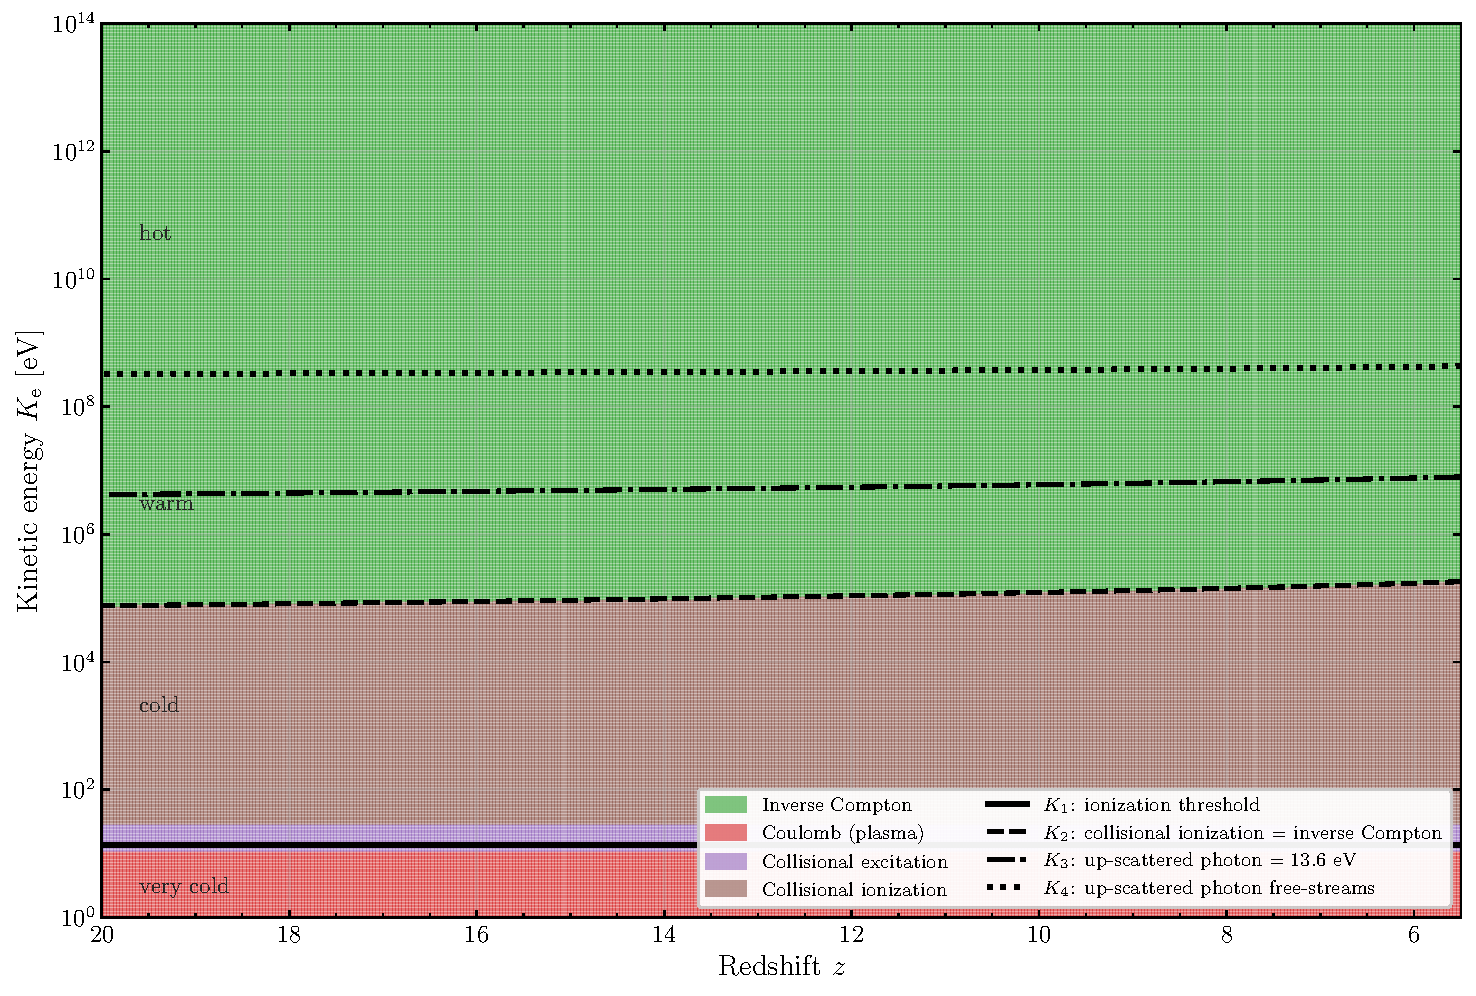
\includegraphics[width=0.82\textwidth]{figures/fig02_phase_space.pdf}
\caption{Dominant energy-loss channel in the $(z,\Ke)$ plane over
$5.5 \le z \le 20$ (shaded), with the four computed boundaries of
Table~\ref{tab:bins} overlaid: $K_1$ the ionization threshold, $K_2$ the
collisional-ionization/inverse-Compton crossover, $K_3$ the energy at which
up-scattered CMB photons become ionizing, and $K_4$ the energy above which
those photons free-stream. $K_3$ subdivides the warm regime rather than
bounding it.}
\label{fig:phase}
\end{figure*}

\begin{table}[t]
\centering
\caption{Computed boundaries of the four regimes, and the photon energy
$E_\gamma^{\mathrm{free}}$ at which the proper mean free path equals the Hubble
radius $c/H(z)$. All electron energies in eV.}
\label{tab:bins}
\small
\begin{tabular}{lccccc}
\toprule
$z$ & $K_1$ & $K_2$ & $K_3$ & $E_\gamma^{\mathrm{free}}$ & $K_4$ \\
\midrule
$20.0$ & $13.61$ & $7.60\times10^{4}$ & $4.20\times10^{6}$ & $1820$ & $3.25\times10^{8}$ \\
$15.0$ & $13.61$ & $9.32\times10^{4}$ & $4.88\times10^{6}$ & $1550$ & $3.43\times10^{8}$ \\
$10.0$ & $13.61$ & $1.23\times10^{5}$ & $5.99\times10^{6}$ & $1272$ & $3.75\times10^{8}$ \\
$8.0$  & $13.61$ & $1.43\times10^{5}$ & $6.67\times10^{6}$ & $1151$ & $3.94\times10^{8}$ \\
$5.5$  & $13.61$ & $1.82\times10^{5}$ & $7.93\times10^{6}$ & $983$  & $4.29\times10^{8}$ \\
\bottomrule
\end{tabular}
\end{table}

\subsection{Where the energy actually goes}

Knowing which channel is fastest at a given instant is not the same as knowing
where an electron's energy ends up, because the electron sweeps downwards
through the regimes as it cools. Figure~\ref{fig:budget} therefore shows the
integrated budget: the fraction of $\Kini$ that each channel has absorbed by
the time the electron reaches the thermal floor. The picture it gives is
cleaner than Fig.~\ref{fig:rates} might suggest. For
$\Kini \lesssim 10^{4}\ \mathrm{eV}$ the budget is essentially independent of
both $\Kini$ and $\zi$ and is shared between collisional ionization
($\simeq 0.48$--$0.72$) and collisional excitation ($\simeq 0.26$--$0.40$),
with Coulomb heating taking $\simeq 0.12$ at $100\ \mathrm{eV}$ and falling
rapidly. For $\Kini \gtrsim 10^{7}\ \mathrm{eV}$ inverse Compton takes
everything: $f_{\mathrm{IC}} = 0.93$ at $10\ \mathrm{MeV}$ and
$>\!0.99$ above $100\ \mathrm{MeV}$ ($\zi = 10$).

The transition between these two limits is narrow, and it is where the
physically interesting behaviour lives. At $\Kini = 10^{5}\ \mathrm{eV}$ and
$\zi = 10$ the split is $f_{\mathrm{ion}} = 0.61$, $f_{\mathrm{exc}} = 0.18$,
$f_{\mathrm{IC}} = 0.17$; one decade higher, at $10^{6}\ \mathrm{eV}$, it has
already inverted to $f_{\mathrm{IC}} = 0.66$, $f_{\mathrm{ion}} = 0.19$. Two
decades in injection energy therefore convert the electron from a device that
deposits two-thirds of its energy directly into the atomic gas to one that
radiates two-thirds of it away. Everything that follows about the ionizing
efficiency of cosmic-ray electrons is a consequence of this inversion.

\begin{figure*}[t]
\centering
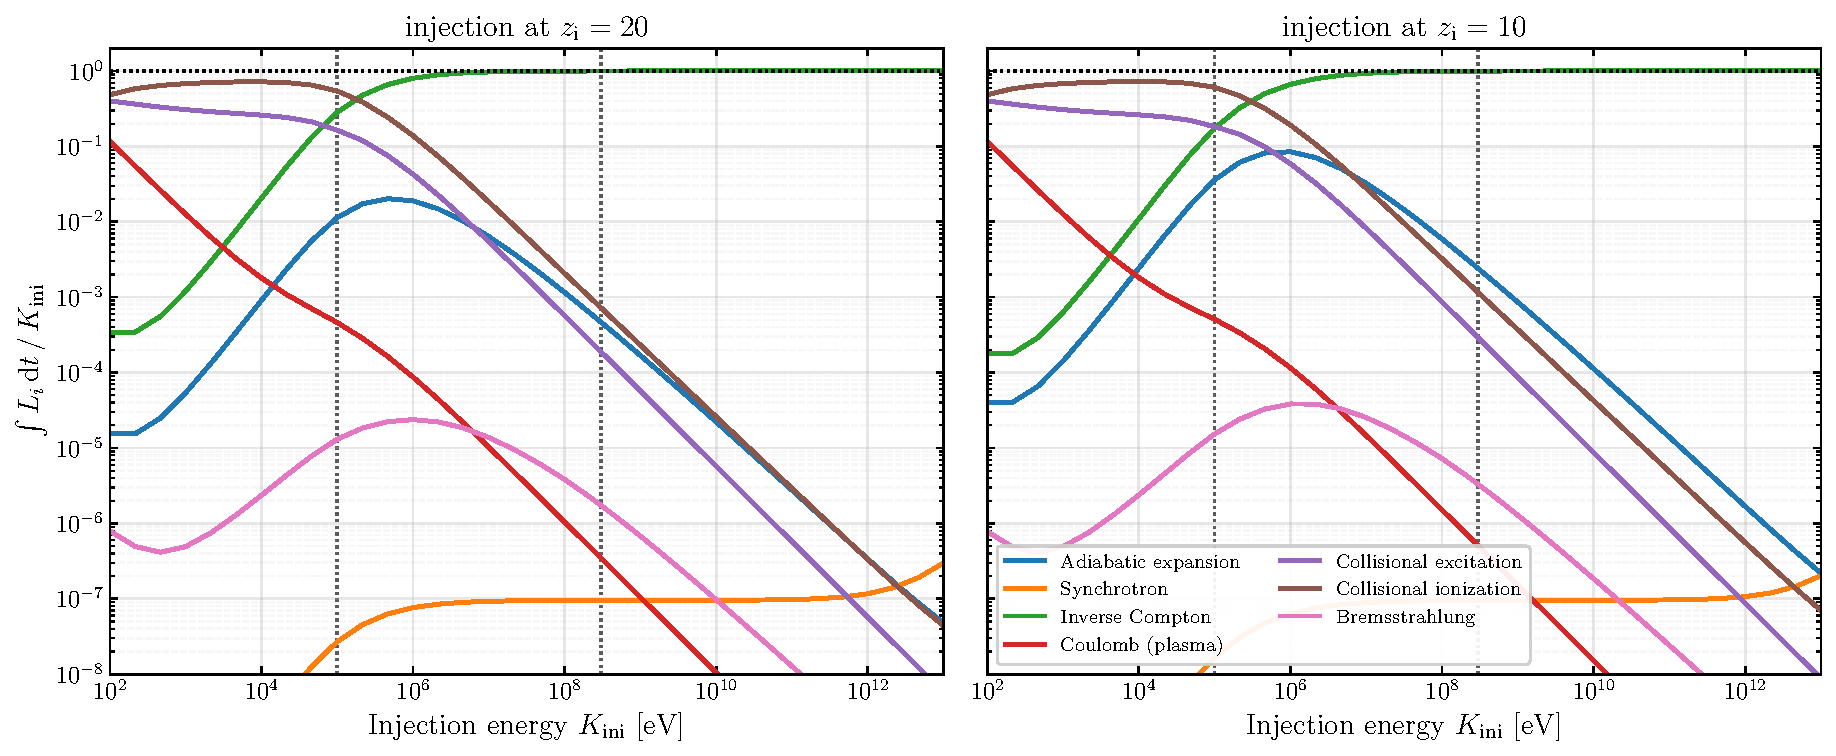
\includegraphics[width=\textwidth]{figures/fig04_energy_budget.pdf}
\caption{Fraction of the injected kinetic energy absorbed by each channel,
$\int L_i\,\mathrm{d}t/\Kini$, integrated along the true trajectory from
injection to thermalization, for $\zi = 20$ (left) and $\zi = 10$ (right).
Dotted vertical lines as in Fig.~\ref{fig:rates}.}
\label{fig:budget}
\end{figure*}

% =====================================================================
\section{Very cold electrons: Coulomb heating}
\label{sec:verycold}
% =====================================================================

\subsection{The only open channel below \texorpdfstring{$10.2\ \mathrm{eV}$}{10.2 eV}}

Below the Lyman-$\alpha$ excitation threshold at $10.204\ \mathrm{eV}$ no
inelastic channel involving neutral hydrogen is kinematically accessible: the
electron cannot excite an atom, cannot ionize one, and radiates negligibly. The
only remaining sink is elastic and quasi-elastic Coulomb scattering off the
residual free electrons of the partially ionized plasma, which converts the
cosmic-ray electron's kinetic energy directly into thermal energy of the gas
\citep{Gould1972}. This is visible in Fig.~\ref{fig:rates} as the red curve
that rises towards low energies and is the unique surviving channel below
$K_1$, and in Fig.~\ref{fig:phase} as the red band at the bottom of the plane.
Between $10.2$ and $13.6\ \mathrm{eV}$ collisional excitation opens and takes
over, so the strictly Coulomb-only regime is bounded above by the
Lyman-$\alpha$ threshold, exactly as in the conceptual scheme.

The efficiency of this channel is set by the residual ionization fraction, and
this is the one place where the fiducial $x_e = 10^{-4}$ enters a result
directly. The Coulomb rate is proportional to $n_e = x_e n_{\mathrm{HI}}$, so a
medium ten times more ionized heats ten times faster at fixed cosmic-ray
energy. In the integrated budget (Fig.~\ref{fig:budget}) Coulomb losses account
for $\simeq 12\%$ of a $100\ \mathrm{eV}$ electron's energy but only $1.8\times
10^{-3}$ of a $10\ \mathrm{keV}$ one, because a fast electron spends very
little of its life at the low energies where Coulomb scattering competes. Very
cold electrons are thus not a by-product of the cascade of fast ones; they
matter only if the source injects them directly, which is precisely the
regime in which cosmic-ray heating of the early IGM has been found to be
significant \citep{Sazonov2015,Leite2017}.

\subsection{Thermal response: heating up, recombining less}
\label{sec:heating}

The consequence of that heating is twofold, and the two effects reinforce each
other. The first is direct: raising the IGM kinetic temperature raises the
21-cm spin temperature above the CMB temperature and switches the global signal
from absorption to emission. This is the effect that current cosmic-ray
calculations were designed to capture, and it is substantial ---
$\Delta T \simeq 10$--$200\ \mathrm{K}$ by $z = 10$ for plausible injection
spectra \citep{Leite2017}, enough to satisfy the HERA requirement that the gas
be above the adiabatic floor by $z = 10.4$ \citep{HERA2023} without invoking
X-ray binaries. Because the heating is deposited close to its sources it is
also spatially structured, which enhances small-scale 21-cm power relative to
X-ray heating models \citep{GesseyJones2023}, although for the diffusion
coefficients usually assumed the structure washes out and the heating is
effectively uniform at high redshift \citep{Jana2018}.

The second consequence is indirect but bears directly on the reionization
budget. The case-B recombination coefficient of hydrogen scales approximately
as $\alpha_B \propto T^{-0.7}$, so a medium heated from the adiabatic floor of
a few kelvin to $10^{2}$--$10^{4}\ \mathrm{K}$ recombines more slowly, and each
ionizing photon produced by any source --- stellar or otherwise --- goes
further. The magnitude of this effect must be stated carefully: cosmic rays
heat the neutral gas, whereas recombinations occur in the H\,\textsc{ii}
regions, which photoionization already holds near $10^{4}\ \mathrm{K}$, so an
extra $\Delta T \lesssim 200\ \mathrm{K}$ changes $\alpha_B$ there by
$\lesssim\!1.4\%$; the larger lever is the pre-heating of the gas
\emph{before} it is ionized, discussed in Sect.~\ref{sec:budget}. Measured IGM temperatures at the tail end of reionization,
$T_0 \simeq 1.0$--$1.2\times10^{4}\ \mathrm{K}$ at $z = 5.4$--$5.8$
\citep{Gaikwad2020}, confirm that the gas is indeed hot by then. Cosmic-ray
heating therefore contributes to the ionization budget through a channel that
is entirely distinct from producing free electrons itself: by suppressing the
sink term. This is worth separating explicitly, because it means the total
cosmic-ray effect on reionization is not simply the number of ionizations the
cosmic rays themselves cause.

% =====================================================================
\section{Cold electrons: direct collisional ionization}
\label{sec:cold}
% =====================================================================

\subsection{The ionization yield per injected electron}

Between $K_1$ and $K_2$ collisional ionization of neutral hydrogen is the
dominant loss channel, and the electron deposits its energy by making free
electrons directly. Counting them requires following not only the primary but
every generation it spawns, because each ionizing collision ejects a secondary
of energy $\epsilon$ and any secondary with $\epsilon > 13.6\ \mathrm{eV}$
ionizes in turn. We therefore solve the fixed point
\begin{equation}
\frac{\mathrm{d}Y}{\mathrm{d}t} = n_{\mathrm{HI}}\,v\,
\sigma_{\mathrm{ion}}(\Ke)\Bigl[\,1 + \langle Y(\epsilon, z)\rangle_{p(\epsilon|\Ke)}\Bigr],
\label{eq:cascade}
\end{equation}
marching upward in energy (a secondary always has
$\epsilon \le (\Ke - B)/2 < \Ke$, so the recursion is causal) and integrating
\emph{every} generation along its own cosmological trajectory with the same
seven-channel loss model. No ceiling is placed on the secondary energy: a
secondary born above $K_4$ loses its energy to escaping photons exactly as a
primary does.

The secondary spectrum $p(\epsilon|\Ke)$ is the BEB singly-differential cross
section \citep{KimRudd1994} rebuilt from the same dipole coefficients that
generate the total RBEB cross-section of \citet{Kim2000}, so that the
differential and integral descriptions are one and the same physics; for
hydrogen it gives $N_i = 0.43431$, and integrating it reproduces the total
cross-section to $0.01\%$ below $300\ \mathrm{eV}$ and $2.6\%$ at
$10\ \mathrm{keV}$. This matters because the spectrum is energy dependent:
the mean secondary energy runs from $1.5\ \mathrm{eV}$ at
$\Ke = 20\ \mathrm{eV}$ to $9.7$, $21.8$ and $40.4\ \mathrm{eV}$ at $100\
\mathrm{eV}$, $1\ \mathrm{keV}$ and $100\ \mathrm{keV}$, so successive
generations are launched into different parts of the yield curve, and
$\langle Y(\epsilon)\rangle \ne Y(\langle\epsilon\rangle)$ wherever $Y$ is
non-linear.

\subsection{The yield is not proportional to the injected energy}

Figure~\ref{fig:yield} and Table~\ref{tab:cascade} give the result. The shower
is not a small correction: it multiplies the yield by $1.02$ at
$100\ \mathrm{eV}$, $1.25$ at $1\ \mathrm{keV}$, $1.57$ at $12\ \mathrm{keV}$
and $\simeq\!2.0$ above $10\ \mathrm{MeV}$, reaching $2.3$--$2.5$ at
$\mathrm{TeV}$ energies, and it is the generations beyond the first that carry
the agreement with the Monte Carlo literature. Writing the derived quantity
$W(\Kini) = \Kini/Y$ makes the point that no single number reproduces the
yield: $W$ falls from $40.1\ \mathrm{eV}$ at $100\ \mathrm{eV}$ to a broad
minimum of $35.4\ \mathrm{eV}$ near $1\ \mathrm{keV}$, is back to
$52.8\ \mathrm{eV}$ at $110\ \mathrm{keV}$, and then rises without limit ---
$208\ \mathrm{eV}$ at $1\ \mathrm{MeV}$, $1.5\times10^{3}$ at
$10\ \mathrm{MeV}$, $1.4\times10^{8}$ at $1\ \mathrm{TeV}$. Any calculation
that adopts $Y = \Kini/W$ with a constant $W$ is therefore wrong by orders of
magnitude for $\Kini \gtrsim 1\ \mathrm{MeV}$, and the error is in the
non-conservative direction.

The minimum is worth isolating, because it is where our calculation makes
contact with the literature. At the minimum the deposition fractions are
$f_{\mathrm{ion}} = 0.38$, $f_{\mathrm{exc}} = 0.42$ and
$f_{\mathrm{heat}} = 0.19$, and $W = 35.4\ \mathrm{eV}$ at both $\zi = 20$ and
$\zi = 10$ to three significant figures --- the $x_e \rightarrow 0$ limit of
\citet{Shull1985} and \citet{Furlanetto2010}, recovered here from atomic
cross-sections alone with no fitted parameter. That agreement also disposes of
the value of $20.8\ \mathrm{eV}$ sometimes quoted as a rule of thumb: it would
require $f_{\mathrm{ion}} = B/20.8 = 0.65$, far above the $\simeq\!0.39$
ceiling a neutral medium allows, and in a neutral IGM the Lyman-band photons
produced by the excitation channel cannot ionize $\mathrm{H}(1s)$ at all.
It coincides instead with $B + \langle\epsilon\rangle$ at
$\Ke = 61\ \mathrm{eV}$, that is with the energy a slow primary loses per
ionizing collision --- a stopping-power quantity, not a deposition
$W$-value.

\begin{table}[t]
\centering
\caption{Cascade ionization yield $Y$ per injected electron, the primary-only
count $N_1$ for comparison, and the derived $W = \Kini/Y$. $Y$ includes every
generation of the shower, each integrated along its own trajectory.}
\label{tab:cascade}
\small
\begin{tabular}{lcccc}
\toprule
$\Kini$ [eV] & $\zi$ & $N_1$ & $Y$ & $W = \Kini/Y$ [eV] \\
\midrule
$1.1\times10^{2}$ & $20$ & $2.60$ & $2.65$ & $40.1$ \\
$1.0\times10^{3}$ & $20$ & $22.6$ & $28.2$ & $35.4$ \\
$1.2\times10^{4}$ & $20$ & $206$  & $323$  & $37.1$ \\
$1.1\times10^{5}$ & $20$ & $1163$ & $2089$ & $52.8$ \\
$1.0\times10^{6}$ & $20$ & $2568$ & $4880$ & $208$ \\
$8.6\times10^{7}$ & $20$ & $3276$ & $6667$ & $1.30\times10^{4}$ \\
$1.1\times10^{12}$& $20$ & $3293$ & $7648$ & $1.42\times10^{8}$ \\
\midrule
$1.1\times10^{2}$ & $10$ & $2.60$ & $2.65$ & $40.1$ \\
$1.0\times10^{3}$ & $10$ & $22.6$ & $28.3$ & $35.4$ \\
$1.2\times10^{4}$ & $10$ & $208$  & $326$  & $36.7$ \\
$1.1\times10^{5}$ & $10$ & $1307$ & $2361$ & $46.8$ \\
$1.0\times10^{6}$ & $10$ & $3499$ & $6755$ & $151$ \\
$8.6\times10^{7}$ & $10$ & $4894$ & $10327$& $8.36\times10^{3}$ \\
$1.1\times10^{12}$& $10$ & $4930$ & $12369$& $8.77\times10^{7}$ \\
\bottomrule
\end{tabular}
\end{table}

\begin{figure*}[t]
\centering
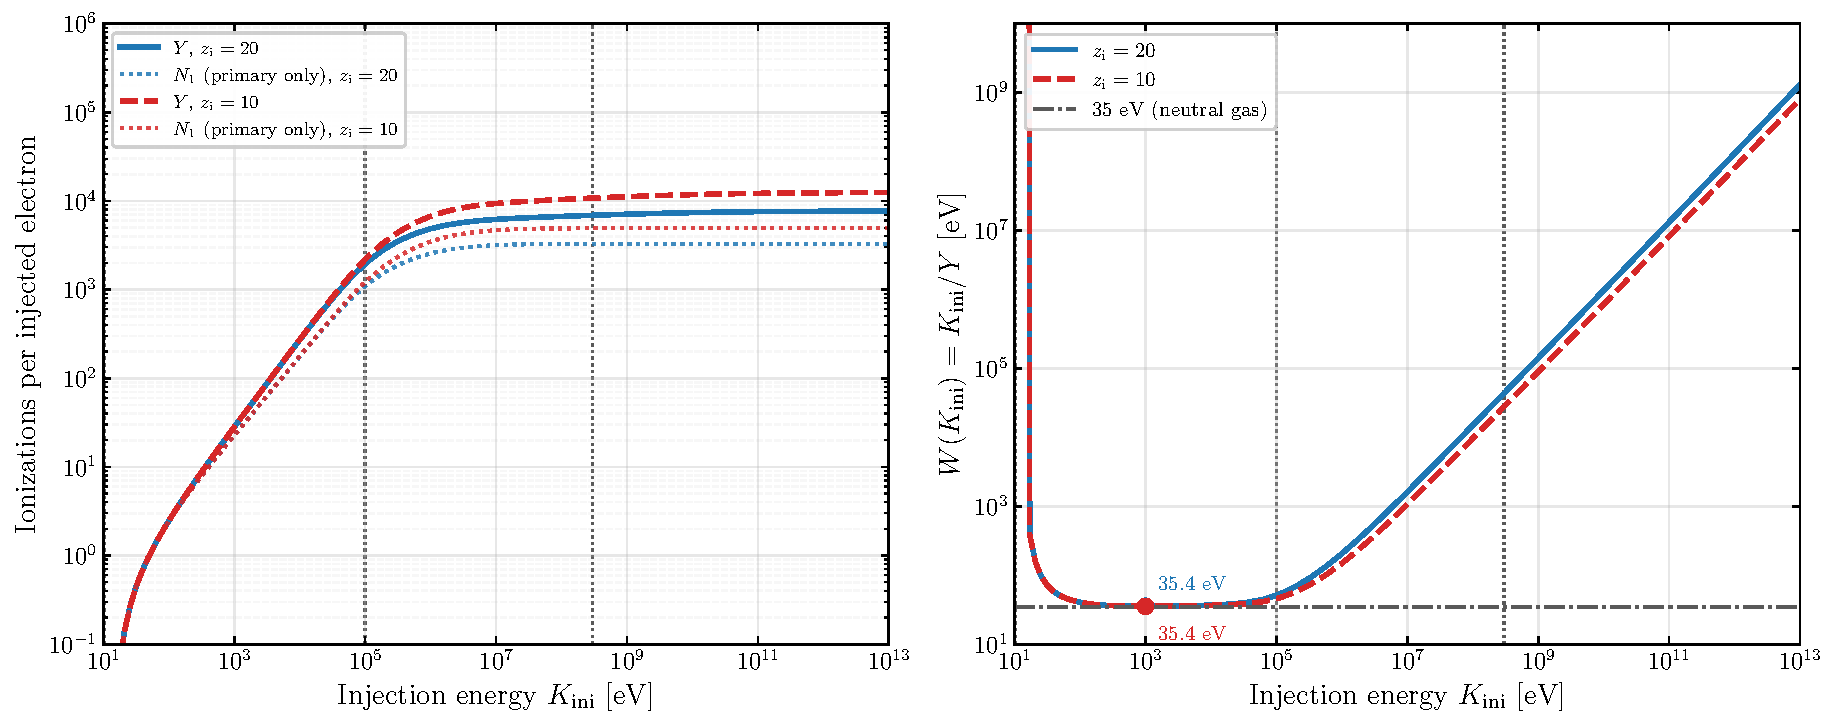
\includegraphics[width=\textwidth]{figures/fig05_ionization_yield.pdf}
\caption{Left: ionizations produced by one injected electron. Solid and dashed
curves give the cascade yield $Y$, which includes every generation of the
secondary shower; dotted curves give the primary-only count $N_1$ for
comparison. Right: the derived $W(\Kini) = \Kini/Y$, with its minimum marked.
$W$ is manifestly not a constant --- it has a broad minimum of
$35.4\ \mathrm{eV}$ near $1\ \mathrm{keV}$ and rises without limit above
$\sim\!10^{5}\ \mathrm{eV}$ --- so the yield cannot be written as
$\Kini$ divided by a fixed energy per ionization. Dotted vertical lines mark
the nominal regime boundaries.}
\label{fig:yield}
\end{figure*}

\subsection{Saturation: the ceiling on the yield}

The most consequential feature of Fig.~\ref{fig:yield} is not the near-linear
low-energy regime but its termination. Above
$\Kini \simeq 10^{8}\ \mathrm{eV}$ the yield flattens to
$Y \simeq 7.7\times10^{3}$ for $\zi = 20$ and $1.2\times10^{4}$ for
$\zi = 10$; increasing the injection energy from $10^{8}$ to
$10^{12}\ \mathrm{eV}$ --- four orders of magnitude --- adds only $15$ and
$20\%$ respectively, the residual creep coming from the handful of very
energetic secondaries that each start a shower of their own. Equivalently,
$W$ rises from $35\ \mathrm{eV}$ to $\sim\!10^{8}\ \mathrm{eV}$ across the
same range: a TeV cosmic-ray electron is, per unit energy, a factor
$2\times10^{6}$ less efficient at ionizing hydrogen than a $1\ \mathrm{keV}$
one.

The origin of the ceiling is the competition already visible in
Fig.~\ref{fig:rates}. Above $K_2$ the inverse-Compton rate exceeds the
collisional-ionization rate and grows as $\Ke^{2}$, so the more energy the
electron carries the faster it is stripped by the CMB and the less time it
spends in the energy range where it can ionize atoms. The ceiling is
therefore set not by $\Kini$ but by the number of ionizations accumulated
during the final passage through the cold regime, which is nearly the same for
every electron that enters it from above. That the ceiling is lower at
$\zi = 20$ than at $\zi = 10$ follows from the same argument: at higher
redshift $U_{\mathrm{CMB}}$ is larger by $(21/11)^{4} \simeq 13$, cooling is
correspondingly faster, and the electron passes through the productive window
more quickly.

% =====================================================================
\section{Warm electrons: Compton-mediated ionization}
\label{sec:warm}
% =====================================================================

\subsection{From electron energy to photon energy}

Above $K_2$ the electron no longer ionizes the medium directly in any
significant measure; it up-scatters CMB photons, and whether those photons
ionize anything depends entirely on where they land in energy. This makes the
warm regime qualitatively different from the cold one: the deposition is
non-local, mediated by radiation, and it has an energy threshold of its own.
Between $K_2$ and $K_3$ the up-scattered photons remain below
$13.6\ \mathrm{eV}$ and cannot ionize hydrogen at all. Photons emerging in the
narrow band between $10.2$ and $13.6\ \mathrm{eV}$ are Lyman-series photons and
do useful work --- they couple the 21-cm spin temperature to the gas through
the Wouthuysen--Field effect --- but photons below $10.2\ \mathrm{eV}$ simply
redshift away without interacting. A significant part of the inverse-Compton
budget in the range $10^{5} \lesssim \Kini \lesssim 10^{6.5}\ \mathrm{eV}$ is
therefore lost to the radiation background rather than deposited in the gas.

Above $K_3 \simeq 4$--$8\ \mathrm{MeV}$ the situation changes: the up-scattered
photons are ionizing, and each one that is absorbed liberates a photoelectron
which then re-enters the cascade analysed in Sect.~\ref{sec:cold} at its own
energy. The total ionization count for a warm electron is consequently
$Y^{\mathrm{tot}} = N_\gamma + \sum_j Y(K_j)$, where $N_\gamma$ counts the
primary photoionizations and the sum runs over the photoelectrons, each
contributing according to the same yield curve $Y$ established above. Our
integration follows the collisional cascade but not this photon-mediated
branch, so the yields plotted in Fig.~\ref{fig:yield} are, in the warm regime,
strictly a lower bound; the photon-mediated contribution is
the subject of the follow-up calculation described in
Sect.~\ref{sec:outlook}.

\subsection{Absorption is local}

What makes this channel viable at all is that the photons produced between
$K_3$ and $K_4$ are absorbed essentially where they are made. The left panel of
Fig.~\ref{fig:threshold} shows the proper mean free path of a photon in the
fiducial IGM, computed from the exact hydrogen photoionization cross-section
\citep{Karzas1961} together with the Klein--Nishina cross-section on bound and
free electrons. At $z = 10$ a photon at the ionization threshold travels
$2\times10^{-4}\ \mathrm{Mpc}$ and one at $100\ \mathrm{eV}$ travels
$0.08\ \mathrm{Mpc}$, both utterly negligible compared with the
$217\ \mathrm{Mpc}$ Hubble radius. The steep $E^{-3}$ decline of the
photoionization cross-section means that the medium remains highly opaque
throughout the band that matters.

The consequence is that the warm regime behaves, to a good approximation, like
the cold one with an extra step inserted: energy leaves the electron as
radiation but is redeposited within a distance that is negligible on any
cosmological scale, so the ionizations still occur in the immediate
neighbourhood of the source. This is what justifies treating the warm and cold
contributions on the same footing when they are later summed into a shell
budget (Sect.~\ref{sec:shell}), and it is what fails --- abruptly --- in the
hot regime.

\begin{figure*}[t]
\centering
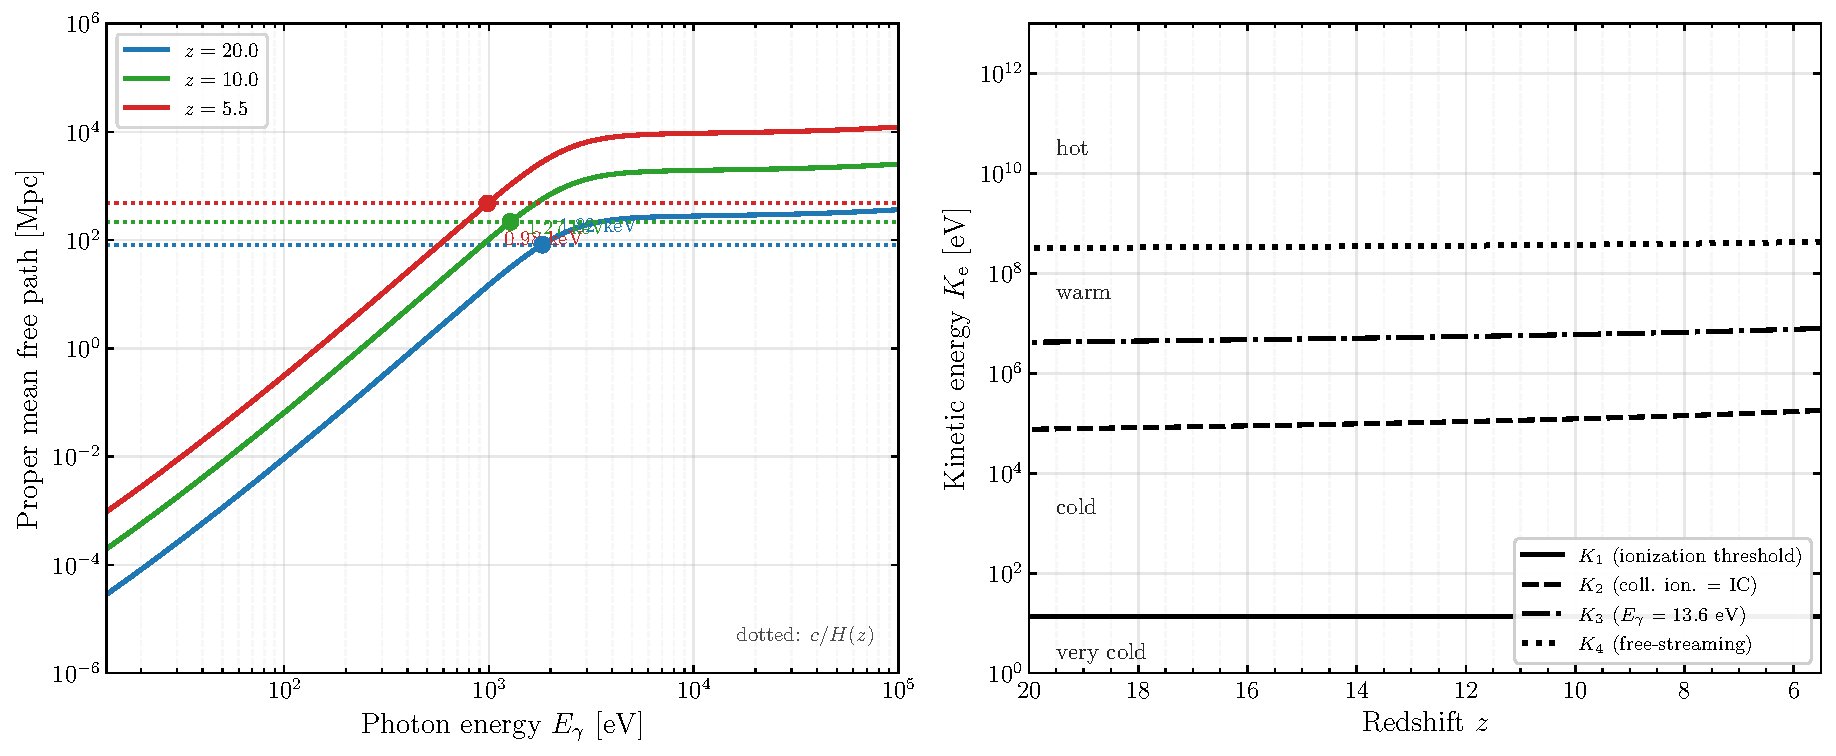
\includegraphics[width=\textwidth]{figures/fig07_thresholds.pdf}
\caption{Left: proper mean free path of a photon in the fiducial IGM at
$z = 20$, $10$ and $5.5$ (solid), including hydrogen photoionization
\citep{Karzas1961} and Klein--Nishina scattering; dotted lines mark the Hubble
radius $c/H(z)$, and the filled circles locate
$E_\gamma^{\mathrm{free}}$, where the two are equal. Right: the resulting
electron-energy boundaries $K_1$--$K_4$ as functions of redshift.}
\label{fig:threshold}
\end{figure*}

% =====================================================================
\section{Hot electrons: energy lost to infinity}
\label{sec:hot}
% =====================================================================

\subsection{The free-streaming threshold}

The hydrogen photoionization cross-section falls as $E_\gamma^{-3}$, so the
opacity of the IGM collapses within a single decade above the threshold, and at
some photon energy the mean free path exceeds the Hubble radius and the photon
ceases to interact with the medium at all. Solving
$\lambda(E_\gamma) = c/H(z)$ with the full opacity gives
$E_\gamma^{\mathrm{free}} = 1.82$, $1.27$ and $0.98\ \mathrm{keV}$ at
$z = 20$, $10$ and $5.5$ (Fig.~\ref{fig:threshold}, left, and
Table~\ref{tab:bins}). The threshold moves to lower energy as the Universe
expands because the density drops faster than the Hubble rate. This is the same
transparency window that governs the energy deposition efficiency of exotic
injections in the dark ages \citep{Slatyer2009,Kanzaki2008,Slatyer2016}, and
its location near $1\ \mathrm{keV}$ is a robust feature of a neutral
hydrogen-dominated medium.

Translating this back into an electron energy through the Compton kinematics
gives the fourth boundary: $K_4 = 3.25\times10^{8}$, $3.75\times10^{8}$ and
$4.29\times10^{8}\ \mathrm{eV}$ at $z = 20$, $10$ and $5.5$. Electrons above
roughly $300\ \mathrm{MeV}$ convert their energy into photons that leave the
medium without depositing anything --- they are, in the language of the
conceptual scheme, lost to infinity. It is worth noting that this boundary is
remarkably flat in redshift, varying by only $32\%$ across a factor of $3.2$ in
$(1+z)$, because the rise in $E_\gamma^{\mathrm{free}}$ with redshift is nearly
compensated by the rise in the CMB photon energy that is being up-scattered.

\subsection{The dominant population is the useless one}

The astrophysical significance of $K_4$ is that it sits well below the energies
at which cosmic-ray accelerators deposit most of their power. A DSA spectrum
$\mathrm{d}N/\mathrm{d}K \propto K^{-p}$ with $p \simeq 2$
\citep{Park2015,Ruszkowski2023} distributes energy equally per logarithmic
interval, so an accelerator operating from GeV to TeV places the overwhelming
majority of its \emph{energy} above $K_4$ even though most of its
\emph{particles} may lie below. For those electrons the ionization yield is not
merely reduced, it is capped at the plateau of Sect.~\ref{sec:cold},
and the entire excess is radiated into a background that the IGM cannot see.

This is the central negative result of the paper, and it is worth stating
precisely, because the four boundaries do not carve out a single efficient
window but two productive bands separated by a dead one. Below $K_2$ the
electron ionizes directly at $W \simeq 35$--$53\ \mathrm{eV}$. Between
$K_2$ and $K_3$ inverse Compton takes the energy but the up-scattered photons
are below $13.6\ \mathrm{eV}$: apart from the thin Lyman-band slice noted in
Sect.~\ref{sec:warm}, that energy is lost to the sub-ionizing radiation
background, and this band is the least productive part of the whole plane.
Between $K_3$ and $K_4$ the photons are ionizing and are reabsorbed within a
negligible distance, so the energy returns to the gas as photoionizations ---
a contribution our direct-only integration does not count, which is why the
plateau in Fig.~\ref{fig:yield} understates the true yield there. Above $K_4$
nothing is recovered at all. Since a DSA spectrum with $p \simeq 2$ places most
of its energy above $K_4$, any scenario proposing cosmic-ray electrons as a significant reionization
source must explain not merely how enough energy is injected, but how it is
kept out of the escaping band --- either by a soft spectrum or by a cutoff
below $\sim\!400\ \mathrm{MeV}$. We return to this in
Sect.~\ref{sec:scenarios}.

% =====================================================================
\section{Ionizations per spherical shell per \texorpdfstring{$\Delta z$}{Dz}}
\label{sec:shell}
% =====================================================================

\subsection{Cooling time and the redshift interval}

Having established the yield per electron, the next step of the scheme is to
distribute those ionizations in space and time --- to convert
$Y(\Kini,\zi)$ into a number of ionizations per spherical shell per
redshift interval $\Delta z$. The temporal part is straightforward, because the
integration already returns the redshift at which each electron thermalizes.
Figure~\ref{fig:cooling} shows $\Ke$ against $\Delta z = \zi - z$ and makes the
timescales explicit. At $\zi = 10$, an electron injected at
$10^{5}\ \mathrm{eV}$ thermalizes by $\Delta z = 0.40$, one at
$10^{6}\ \mathrm{eV}$ by $\Delta z = 1.82$, and one at
$10^{12}\ \mathrm{eV}$ by $\Delta z = 2.85$. At $\zi = 20$ the same energies
thermalize by $\Delta z = 0.25$, $0.89$ and $1.23$ respectively.

Two features of these numbers matter for the shell construction. First, the
thermalization redshift saturates with injection energy for exactly the reason
the yield does: above $K_4$ the extra energy is dumped into escaping photons on
a timescale that is short compared with the Hubble time, so a TeV electron and
a $100\ \mathrm{MeV}$ electron reach the thermal floor at almost the same
epoch. Second, cooling is markedly faster at high redshift, so the deposition
is more sharply localized in $\Delta z$ at $z = 20$ than at $z = 10$. A shell
budget constructed with a fixed $\Delta z$ will therefore resolve the injection
history well at early times and poorly at late times; the natural choice is a
$\Delta z$ that tracks the cooling time, which for our purposes means
$\Delta z \lesssim 0.3$ at $z \gtrsim 15$ and $\Delta z \lesssim 1$ at
$z \sim 10$.

\begin{figure*}[t]
\centering
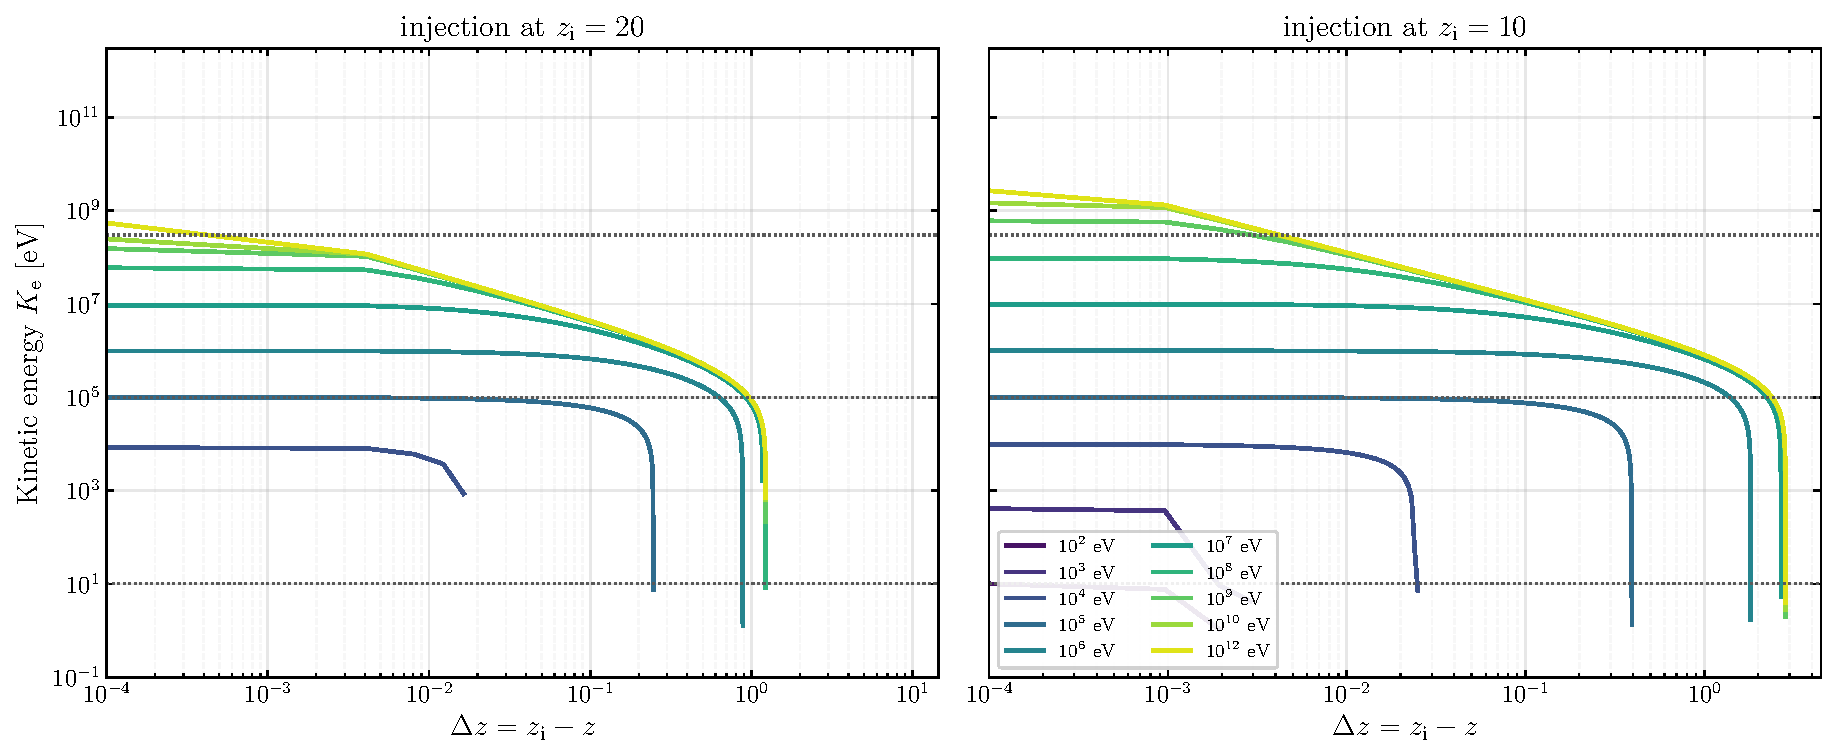
\includegraphics[width=\textwidth]{figures/fig03_cooling_histories.pdf}
\caption{Kinetic energy against elapsed redshift interval
$\Delta z = \zi - z$ for electrons injected at $\zi = 20$ (left) and
$\zi = 10$ (right), for injection energies from $10^{2}$ to
$10^{12}\ \mathrm{eV}$. Curves terminate at the thermal floor
$\tfrac{3}{2}kT_{\mathrm{CMB}}(z)$. Dotted horizontal lines mark the nominal
regime boundaries.}
\label{fig:cooling}
\end{figure*}

\subsection{The radial extent is set by transport, not by cooling}

The spatial part is much less straightforward, and it is important to be
explicit about what our calculation does and does not determine.
Figure~\ref{fig:distance} shows the kinetic energy against the comoving path
length $\chi = \int v (1+z)\,\mathrm{d}t$ accumulated along the trajectory. The
path length saturates in the same way the other quantities do: an electron
injected at $10^{5}\ \mathrm{eV}$ traverses $8.0$ comoving Mpc before
thermalizing, one at $10^{6}\ \mathrm{eV}$ traverses $49.6\ \mathrm{Mpc}$, and
everything above $10^{8}\ \mathrm{eV}$ traverses $78.1\ \mathrm{Mpc}$,
against a comoving light-travel distance of $2757\ \mathrm{Mpc}$ from
$z = 20$ to $z = 5.5$.

These path lengths are emphatically \emph{not} shell radii. As noted in
Sect.~\ref{sec:method}, the gyroradius in the fiducial field is
$10^{-8}$--$10^{-2}\ \mathrm{pc}$, some ten orders of magnitude below the path
length, so the electron does not travel in a straight line: it spirals along a
field line and its displacement from the injection site is governed by the
cross-field diffusion coefficient, not by how far it has flown. The correct
statement is that the path length is a rigorous \emph{upper bound} on the shell
radius, saturating at $\sim\!78$ comoving Mpc, and that the actual radius
requires a transport model. This is precisely the quantity that controls
whether cosmic-ray heating is patchy or uniform: \citet{Jana2018} find that
inhomogeneous deposition requires $D \lesssim 10^{26}\ \mathrm{cm^{2}\,s^{-1}}$
at $z \sim 10$, and that for typical values the heating is uniform. Because
the ionization we compute is deposited by the same particles, the same
criterion applies to it, and we adopt the uniform-deposition limit in what
follows.

\begin{figure}[t]
\centering
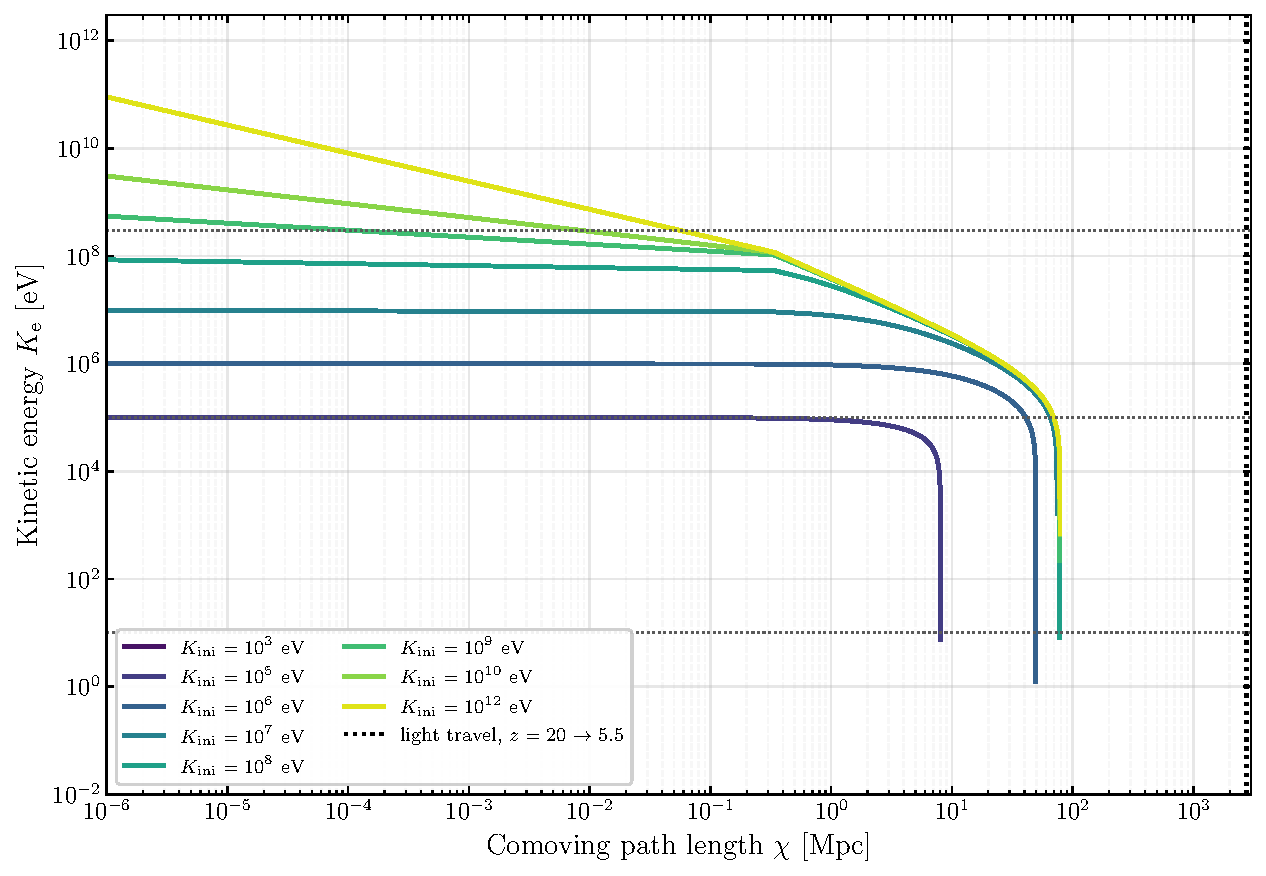
\includegraphics[width=\columnwidth]{figures/fig06_energy_vs_distance.pdf}
\caption{Kinetic energy against comoving path length
$\chi = \int v(1+z)\,\mathrm{d}t$ for electrons injected at $\zi = 20$. The
path length saturates near $78$ comoving Mpc for all
$\Kini \gtrsim 10^{8}\ \mathrm{eV}$. Because the gyroradius is smaller by ten
orders of magnitude, this is an upper bound on the displacement, not the
displacement itself.}
\label{fig:distance}
\end{figure}

% =====================================================================
\section{Discussion}
% =====================================================================

\subsection{Estimating the global contribution}
\label{sec:global}

The global ionization budget follows from the per-electron yield by weighting
it with the injection spectrum. Writing the number of electrons injected per
unit comoving volume per unit energy as
$\mathrm{d}n/\mathrm{d}\Kini = A\,\Kini^{-p}$ between $K_{\min}$ and
$K_{\max}$, the number of ionizations per unit comoving volume is
$n_{\mathrm{ion}} = \int A \Kini^{-p} Y(\Kini)\,\mathrm{d}\Kini$, and the
useful figure of merit is the spectrum-averaged energy per ionization
\begin{equation}
\overline{W}(p) \;=\;
\frac{\displaystyle\int_{K_{\min}}^{K_{\max}} \Kini^{1-p}\,\mathrm{d}\Kini}
     {\displaystyle\int_{K_{\min}}^{K_{\max}} \Kini^{-p}\,Y(\Kini)\,\mathrm{d}\Kini},
\label{eq:Wbar}
\end{equation}
which converts a cosmic-ray electron energy density directly into an ionization
density. The shape of $Y(\Kini)$ established in Sect.~\ref{sec:cold} ---
close to linear up to $\sim\!10^{5}\ \mathrm{eV}$, then bending over and
flattening above $\sim\!10^{8}\ \mathrm{eV}$ --- makes the behaviour of
Eq.~(\ref{eq:Wbar}) easy to anticipate. For $p > 2$ both integrals are dominated by $K_{\min}$,
the flattening is never sampled, and $\overline{W}$ tends to the
low-energy plateau of $W(\Kini)$, $\simeq\!37\ \mathrm{eV}$. For $p < 2$ the numerator is dominated by $K_{\max}$ while
the denominator saturates, so $\overline{W}$ grows as $K_{\max}^{2-p}$. The
canonical DSA value $p = 2$ sits exactly at the transition, where
$\overline{W}$ grows only logarithmically in the dynamic range of the
accelerator.

Table~\ref{tab:Wbar} evaluates Eq.~(\ref{eq:Wbar}) numerically on the yield
curves of Fig.~\ref{fig:yield}, taking $K_{\min} = 100\ \mathrm{eV}$ and
$K_{\max} = 1\ \mathrm{TeV}$. The
anticipated behaviour is borne out with some force. Between $p = 2.5$ and
$p = 1.8$ --- a range comfortably inside the spread of spectral indices that
real accelerators produce --- the spectrum-averaged energy per ionization
degrades by a factor of $21$, from $37.6$ to $804\ \mathrm{eV}$, and the
comoving cosmic-ray electron energy density required to supply one ionization
per hydrogen atom rises correspondingly from
$1.2\times10^{-17}$ to $2.5\times10^{-16}\ \mathrm{erg\,cm^{-3}}$. The
dependence on $\zi$ is negligible by comparison, below $11\%$ across the whole
table.
The global contribution of cosmic-ray electrons to reionization is therefore
controlled almost entirely by the softness of the injection spectrum, and
hardly at all by $K_{\max}$, by the injection redshift, or by the total energy
above a GeV. This inverts the usual intuition that more energetic accelerators
are more effective, and it explains why the hadronic studies cited in Sect.~1
reached a negative verdict on ionization while reaching a positive one on
heating: the proton spectra they adopt place their energy at exactly the
energies where the leptonic yield saturates. Two caveats should be attached to
Table~\ref{tab:Wbar}. It counts collisional ionization only, so it still omits
the photon-mediated ionizations of the band $K_3 < \Kini < K_4$
(Sect.~\ref{sec:warm}); since the integrals for $p < 2$ are dominated by
precisely that band, the $p = 1.8$ entry should be read as a conservative
worst case rather than an estimate. It also requires only one ionization per
atom, neglecting recombinations, so the energy densities quoted are floors. The photon-mediated warm-regime
contribution of Sect.~\ref{sec:warm} and a full recombination bookkeeping are
deferred to the companion paper.

\begin{table}[t]
\centering
\caption{Spectrum-averaged energy per ionization $\overline{W}$ from
Eq.~(\ref{eq:Wbar}) for an injection spectrum
$\mathrm{d}n/\mathrm{d}\Kini \propto \Kini^{-p}$ with
$K_{\min} = 100\ \mathrm{eV}$ and $K_{\max} = 1\ \mathrm{TeV}$, and the
comoving cosmic-ray electron energy density $\varepsilon_{\mathrm{CR}} =
n_{\mathrm{H}}\overline{W}$ needed to supply one ionization per hydrogen atom
($n_{\mathrm{H}} = 1.94\times10^{-7}\ \mathrm{cm^{-3}}$ comoving).}
\label{tab:Wbar}
\small
\begin{tabular}{lcccc}
\toprule
 & \multicolumn{2}{c}{$\zi = 20$} & \multicolumn{2}{c}{$\zi = 10$} \\
\cmidrule(lr){2-3}\cmidrule(lr){4-5}
$p$ & $\overline{W}$ & $\varepsilon_{\mathrm{CR}}$
    & $\overline{W}$ & $\varepsilon_{\mathrm{CR}}$ \\
    & [eV] & [erg\,cm$^{-3}$] & [eV] & [erg\,cm$^{-3}$] \\
\midrule
$1.8$ & $888$  & $2.8\times10^{-16}$ & $804$  & $2.5\times10^{-16}$ \\
$2.0$ & $107$  & $3.3\times10^{-17}$ & $102$  & $3.2\times10^{-17}$ \\
$2.2$ & $46.3$ & $1.4\times10^{-17}$ & $45.3$ & $1.4\times10^{-17}$ \\
$2.5$ & $37.8$ & $1.2\times10^{-17}$ & $37.6$ & $1.2\times10^{-17}$ \\
$3.0$ & $37.4$ & $1.2\times10^{-17}$ & $37.4$ & $1.2\times10^{-17}$ \\
\bottomrule
\end{tabular}
\end{table}

\subsection{Which scenarios are worth exploring}
\label{sec:scenarios}

Equation~(\ref{eq:Wbar}) is, read differently, a design specification for the
accelerator. To make cosmic-ray electrons a competitive ionizing source one
needs an injection spectrum that is steep ($p \gtrsim 2.2$), that extends down
to $K_{\min}$ of order tens of eV rather than being cut off at MeV energies,
and that operates at a redshift where the surrounding medium is still neutral
enough to absorb the resulting photons. The first two requirements point away
from strong supernova blast waves --- which are efficient precisely because
they produce hard spectra extending to high energy --- and towards weaker
shocks, stellar wind termination shocks, and the reacceleration of an existing
low-energy population. The third points to the earlier part of our window.

The redshift dependence works in two opposing directions and this is what makes
the scenario question non-trivial. Injecting earlier means a denser, more
neutral medium, a shorter cooling time and more sharply localized deposition
(Fig.~\ref{fig:cooling}), all of which help; but it also means a
$(1+z)^{4}$-larger CMB energy density, which strengthens the inverse-Compton
sink that steals energy from the ionization channel, and a lower saturation
ceiling ($7.7\times10^{3}$ versus $1.2\times10^{4}$ ionizations per electron
between $\zi = 20$ and $\zi = 10$). The net effect is that the productive
window in $\Kini$ narrows with increasing redshift: $K_2$ falls from
$1.8\times10^{5}$ to $7.6\times10^{4}\ \mathrm{eV}$ between $z = 5.5$ and
$z = 20$ (Table~\ref{tab:bins}). Scenarios that inject at $z \sim 10$--$15$
with a soft spectrum are therefore favoured over both earlier and harder
alternatives, and this is a prediction that a source-population model can be
tested against.

\subsection{Comparison with the reionization history: is it worth exploring?}
\label{sec:outlook}

Set against the observed reionization history, the honest answer is a qualified
yes, for reasons that have more to do with the thermal history than with the
photon budget. Our results confirm, from the leptonic side and with the full
loss physics, the negative verdict that the hadronic literature reached on
ionization \citep{Leite2017}: the flattening of $Y$ above
$\sim\!100\ \mathrm{MeV}$ caps the yield of exactly the particles that carry
the accelerator's energy, and no plausible normalization of a hard spectrum
turns $10^{4}$ ionizations per electron into a competitive share of the
$1.9\times10^{-7}\ \mathrm{cm^{-3}}$ (comoving) of hydrogen that must be
ionized. Cosmic-ray electrons are not going to reionize the Universe on their
own.

What the channel does deliver is a thermal signature at redshifts where the
21-cm experiments are now sensitive, and the same energy budget that makes the
ionization contribution negligible fixes the two quantities together. Because
every fast electron, whatever its injection energy, deposits what it does
deposit through the \emph{same} cold-regime cascade, the heat released per
ionization produced is nearly invariant: our channel-resolved integration of
the cascade gives $6.0$--$9.6\ \mathrm{eV}$ of heat per ionization over
$K_{\mathrm{ini}} = 10^{2}$--$10^{6}\ \mathrm{eV}$, and the value is identical
at $z_i = 10$ and $z_i = 20$ to three significant figures, because the
inverse-Compton leak removes heat and ionizations in the same proportion and
cancels in the ratio. Converting the heat into a temperature rise of a gas with
$1.081$ particles per hydrogen atom, this fixes the number of cosmic-ray
ionizations per hydrogen atom to
\begin{equation}
  \frac{N_{\mathrm{ion}}}{n_{\mathrm{H}}}
  \;=\; \frac{\Delta T}{\left(4.3\text{--}6.9\right)\times10^{4}\ \mathrm{K}} ,
  \label{eq:lock}
\end{equation}
independently of the injection spectrum and of redshift. Equation~(\ref{eq:lock})
is the result that makes the channel testable: a 21-cm measurement of $\Delta T$
is simultaneously a measurement of the leptonic contribution to reionization.

\subsection{Does the leptonic channel narrow or widen the photon budget crisis?}
\label{sec:budget}

The photon budget crisis is the statement that the directly observed galaxy
population already produces too many ionizing photons too early
\citep{Munoz2024}, so a resolution must remove ionizations from the early
Universe or delay them. Equation~(\ref{eq:lock}) says the leptonic channel does
the opposite, and it says by how much. Taking the heating range that the
hadronic calculations obtain for plausible injection spectra,
$\Delta T = 10$--$200\ \mathrm{K}$ at $z = 10$ \citep{Leite2017} --- borrowed
here as a scale, not as a leptonic prediction --- Eq.~(\ref{eq:lock}),
evaluated at the $\Kini \gtrsim 1\ \mathrm{keV}$ end where a cosmic-ray
spectrum carries its energy, gives
$2.3\times10^{-4}$ to $4.6\times10^{-3}$ ionizations per hydrogen atom, i.e.\
$0.02$--$0.5\%$ of reionization, and a Thomson-depth increment
$\delta\tau = 3.5\times10^{-5}$--$7.7\times10^{-4}$, at most a tenth of the
\emph{Planck} uncertainty $\sigma(\tau) = 0.007$ \citep{Planck2020}. Those
numbers are consistent with the 21-cm limits that bracket the same epoch: the
LOFAR upper limits of $\Delta^2_{21} < (54.3\ \mathrm{mK})^2$ at $z \simeq 9.1$
\citep{Mertens2025} disfavour, at $95\%$ credibility, only IGM states with mean
gas temperature below $44\ \mathrm{K}$ and with less than $46\%$ of the volume
ionized or heated \citep{Ghara2025}, so a few tens of kelvin of cosmic-ray
heating is permitted but not required, while the HERA requirement that the gas
exceed the adiabatic floor $T_{\mathrm{ad}} = 2.70\ \mathrm{K}$ by
$z = 10.4$ \citep{HERA2023} is comfortably met at the upper end of the range.

Every other route by which the heat could act on the reionization history runs
in the same direction. Raising the temperature of ionized gas lowers the case-B
recombination coefficient (Sect.~\ref{sec:heating}), which removes sink term and
therefore accelerates reionization; pre-heating the neutral gas also smooths it
in pressure and lowers the recombination-weighted clumping factor
\citep{Pawlik2009}, pushing against the high value
$C = 6.2^{+4.1}_{-2.1}$ that resolves the crisis in the
\citet{Austin2025} analysis of $1721$ galaxies at $5.6 < z < 6.5$. The one
mechanism that would run the other way --- raising the filtering mass so that
star formation in minihaloes is suppressed --- does not apply to the population
at issue: $100\ \mathrm{K}$ of heating gives a Jeans mass
$M_{\mathrm{J}} = 1.5\times10^{6}\ M_\odot$ at $z = 10$, within the halo range
$4.4\times10^{5}$--$1.1\times10^{7}\ M_\odot$ that the SARAS~3 non-detection
already disfavours \citep{Bevins2022}, but some three decades below the
$\gtrsim\!10^{9}\ M_\odot$ hosts of the $M_{\mathrm{UV}} < -15$ galaxies whose
directly measured output creates the tension. The leptonic channel therefore
\emph{widens} the crisis on every channel that acts on the observed population,
by of order $10^{-3}$ of the discrepancy --- which is to say it is
observationally irrelevant to the photon budget and diagnostically valuable to
the thermal history. That is the sense in which the channel is worth pursuing,
and quantifying the joint heating-plus-ionization response against the
$z = 5.3$ end point of \citet{Bosman2022}, the \emph{Planck} optical depth and
the 21-cm limits simultaneously is the question we intend to answer next.

% =====================================================================
\section{Summary}
% =====================================================================

We have integrated the seven simultaneous energy-loss channels of a cosmic-ray
electron in a neutral intergalactic medium from $z = 20$ and $z = 10$ down to
$z = 5.5$, and used the result to quantify the ionizing efficiency of the
leptonic component of cosmic rays during the epoch of reionization. Our main
conclusions are:

\begin{enumerate}
\item The $(z,\Ke)$ plane partitions into four regimes with boundaries that
      follow from the loss physics: $K_1 = 13.6\ \mathrm{eV}$,
      $K_2 = 0.76$--$1.8\times10^{5}\ \mathrm{eV}$,
      $K_3 = 4.2$--$7.9\ \mathrm{MeV}$ and
      $K_4 = 3.2$--$4.3\times10^{8}\ \mathrm{eV}$ (Table~\ref{tab:bins}).
\item Synchrotron losses are irrelevant at all energies and redshifts for
      $B_0 = 1\ \mathrm{nG}$ comoving, since
      $U_B/U_{\mathrm{CMB}} = 9.5\times10^{-8}$ independently of $z$. The
      magnetic field nevertheless dominates transport, the gyroradius being
      ten orders of magnitude below the cooling path length.
\item The ionization yield $Y(\Kini,\zi)$, obtained by solving the cascade
      over every generation of the shower, is not proportional to $\Kini$.
      The derived $W = \Kini/Y$ has a broad minimum of $35.4\ \mathrm{eV}$
      near $1\ \mathrm{keV}$ --- reproducing the $x_e \rightarrow 0$ limit of
      \citet{Shull1985} and \citet{Furlanetto2010} from atomic cross-sections
      alone --- and rises to $208\ \mathrm{eV}$ at $1\ \mathrm{MeV}$ and
      $\sim\!10^{8}\ \mathrm{eV}$ at $1\ \mathrm{TeV}$. $Y$ flattens at
      $7.7\times10^{3}$ ($\zi = 20$) and $1.2\times10^{4}$ ($\zi = 10$)
      ionizations per electron above $10^{8}\ \mathrm{eV}$. The secondary
      shower contributes a factor $1.02$--$2.5$, rising with $\Kini$.
\item Above $K_4$ the up-scattered CMB photons exceed
      $E_\gamma^{\mathrm{free}} \simeq 1\ \mathrm{keV}$, at which the mean free
      path exceeds the Hubble radius, and their energy leaves the medium
      entirely.
\item The contribution is therefore split into two productive bands ---
      $K_1 < \Ke < K_2$ (direct collisional ionization) and
      $K_3 < \Ke < K_4$ (photon-mediated, absorbed locally) --- separated by
      a dead band $K_2 < \Ke < K_3$ in which the up-scattered photons are
      sub-ionizing.
\item The spectrum-averaged energy per ionization, Eq.~(\ref{eq:Wbar}), is
      controlled by the low-energy end of the injection spectrum for
      $p > 2$ and diverges as $K_{\max}^{2-p}$ for $p < 2$: soft spectra
      extending to low energies are the only competitive configuration.
\item Because all the deposited energy passes through the same cold-regime
      cascade, the heat released per ionization is nearly invariant
      ($6.0$--$9.6\ \mathrm{eV}$ over $\Kini = 10^{2}$--$10^{6}\ \mathrm{eV}$,
      and independent of $\zi$ to three significant figures). This locks the
      ionization contribution to the heating, Eq.~(\ref{eq:lock}), so that
      $\Delta T = 10$--$200\ \mathrm{K}$ yields at most
      $4.6\times10^{-3}$ ionizations per hydrogen atom and
      $\delta\tau \lesssim 7.7\times10^{-4}$. The leptonic channel thus
      \emph{widens} rather than relieves the photon budget crisis of
      \citet{Munoz2024}, by a fraction of order $10^{-3}$ of the
      discrepancy, and is best regarded as a probe of the thermal history
      rather than a contributor to the ionizing budget.
\end{enumerate}

\section*{Data and code availability}

All curves shown were generated from a single shared physics module
(\texttt{igm\_losses.py}) and the figure script \texttt{make\_paper\_figures.py}
accompanying this manuscript.

\bibliography{references}

\end{document}
